\documentclass[eng,printmode]{02_class}
\usepackage{geometry}                   % See geometry.pdf to learn the layout options. There are lots.
\usepackage[utf8]{inputenc}
\usepackage[polish]{babel}
\usepackage{polski}

\geometry{letterpaper}                      % ... or a4paper or a5paper or ...
%\geometry{landscape}                   % Activate for for rotated page geometry
%\usepackage[parfill]{parskip}        % Activate to begin paragraphs with an empty line rather than an indent
\usepackage{graphicx}       % Use pdf, png, jpg
\graphicspath{ {images/} }
\usepackage{hyperref}
\usepackage{placeins}

\usepackage{xcolor}
\usepackage{listings}

\lstset{
  breaklines=true,
  basicstyle=\scriptsize,
  frame=single
}
  %this is mainifest file containing all required packages

\title{System do zarządzania zadaniami.}
\author{Sebastian Wilgosz (nr indeksu: 195963), Rafal Sztandera (nr indeksu: XXXXXX) }
\supervisor{dr. mgr inż. Marek Woda}


\newcommand{\R}{I\!\!R} %symbol liczb rzeczywistych, dział‚a tylko w
                        %trybie matematycznym
\newtheorem{theorem}{Twierdzenie}[section]
\field{Informatyka (INF)}
\specialisation{Inżynieria Internetowa (INT)}


\begin{document}
  \maketitle
  \tableofcontents

  \chapter{Wstęp}
  \label{chapter:introduction}
    \section{Cel projektu}
    \label{section:target}
    Celem projektu jest stworzenie systemu mającego rozwiązać problem niskiej efektywności pracy osoby zaangażowanej w wiele różnych projektów, przy użyciu platformy mikroprocesorowej, łacza sieciowego oraz aplikacji serwerowej.

Projekt obejmuje zaprojektowanie i stworzenie autonomicznego urządzenia wspomagającego zarządzenie czasem, serwisu internetowego udostępniającymi te same funkcjonalności w tym tworzenie i prezentację zadań oraz stworzenie i wdrożenie metody synchronizacji danych pomiędzy urządzeniem, a serwisem webowym.

Platforma mikroprocesorowa będzie docelowo wykorzystywana w środowisku domowym jako element wyposażenia. Powinna być łatwo dostępna, dawać możliwość kożystania z niej bez użycia klawiatury, myszy i osobnego ekranu.


    \section{Opis problemu}
    \label{section:problem}
    W dobie dynamicznego wzrostu popularności aplikacji użytkowych na platformy mobilne (rys. \ref{figure:app_download}), oraz w momencie dynamicznego rozwoju technologii związanej z pojęciem Internet of Things, platformy mikroprocesorowe stają przed wyzwaniem zapewnienia funkcjonalności znanych z programów pisanych z myślą o jednostkach stacjonarnych oraz sprostaniem specyficznym wymaganiom dotyczącym rozmiaru, źródła zasilania i obsługi urządzeń nietypowych dla środowiska komputerowego .

Zarówno w przypadku oprogramowania obslugującego platformy mobilne \cite{bib:mobile-challenge}, jak i w przypadku koncepcji Internet of Things, nie zostały ustalone normy standaryzujące proces tworzenia oprogramowania, czy kontrukcji systemów opartych na połączeniu aplikacji webowych i mobilnych lub stacjonarnych. Za cel pracy przyjęto zaprojektowanie platformy mikroprocesorowej będącej zgodną z aktualnymi trendami rozwoju inżynierii internetowej. Wybory i założenia przyjęte podczas prac są tłumaczone, tak, by w oparciu o nich, móc odpowiedzieć na pytanie o granice adaptowalności, skalowalności i możliwości rozwoju systemów wbudowanych jako rozproszonego środowiska działania aplikacji użytkowych.

\begin{figure}[ht]
  \centering
  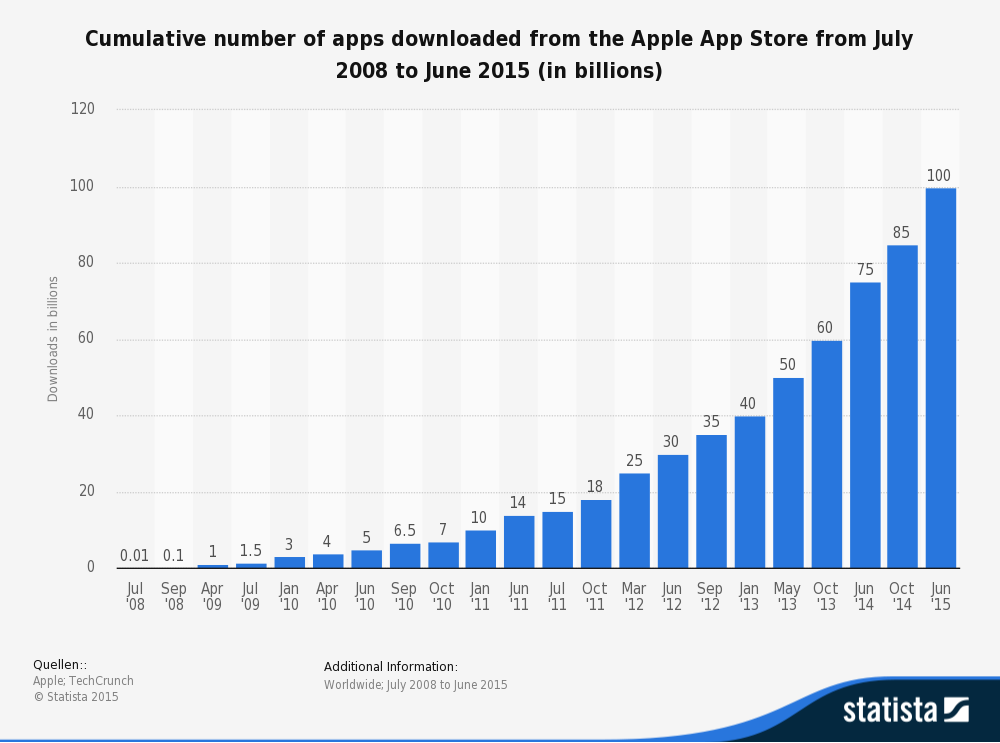
\includegraphics[width=\textwidth]{images/app_downloads.png}
  \caption{Wykres ilości pobrań aplikacji mobilnych dostosowanych do systemu operacyjnego popularnego producenta urządzeń mobilnych na przestrzeni ostatnich 7 lat.}
  \label{figure:app_download}
\end{figure}
\FloatBarrier



\subsection{Wymagania} % (fold)
Określenie wymagań stawianych projektowanemu systemowi zostało oparte o analizę potrzeb użytkownika na przykładzie aplikacji wspomagającej zarządzaniem czasem, oraz ogólno-przyjętymi wyznaczkami jakimi charakteruzją się aplikacje mobilne\cite{bib:mobile-paradigm}.


\label{sub:wymagania}
System przeznaczony jest dla pojedynczych użytkowników, do użytku własnego. Z tej perspektywy ważnymi, ale nie kluczowymi wyznacznikami urządzenia są:
\begin{enumerate}
	\item zapewnienie maksymalnej niezawodności
	\item wytrzymałość na zniszczenia i warunki ekstremalne
	\item możliwość wykonania kopii zapasowej
\end{enumerate}

Kluczowymi cechami platformy, ze względu na swoje przeznaczenie i środowisko pracy są:
\begin{enumerate}
	\item łatwe zarządzanie danymi
	\item trwałość i pewność zapisu
	\item wysoka dostępność do danych
	\item intuicyjność interfejsu aplikacji
	\item łatwa konfiguracja
	\item płynność działania aplikacji
	\item szybka synchronizacja
\end{enumerate}

Wymagania podstawowe stawiane aplikacji:
\begin{enumerate}
	\item możliwość anulowania operacji
	\item możliwość manipulacji danymi (dodawanie/edycja/usuwanie)
	\item interfejs w języku polskim
\end{enumerate}

Dostępność tłumaczy się jako możliwość podglądu zadań z poziomu aplikacji internetowej jak i aplikacji na platformach mikroprocesorowych zsynchronizowanych z aplikacją internetową.

% section wymagania (end)
\subsection{Ograniczenia} % (fold)
\label{sub:ograniczenia}
Ograniczeniem dla projektu są:
\begin{enumerate}
	\item wymiary
	\subitem platforma mikroprocesorowa powinna być możliwie płaska, oraz posiadać duży ekran dotykowy
	\item zasilanie
	\subitem systemy wbudowane wymagają specjalnego zasilania
	\item dostęp do internetu
	\subitem internet jest niezbędny do dwukierunkowej synchronizacji danych z serwerem
\end{enumerate}

Ograniczeniem dla projektu w przyszłości mogą być:
\begin{enumerate}
	\item przepisy regulujące kwestie związane z używaniem urządzeń elektrycznych w określonym środowisku (np. łazienka)
\end{enumerate}


    \section{Opis rozwiązania i wykorzystanych technologii}
    \label{section:solution}
    \subsection{Aplikacja serwerowa}

Do zaimplementowania aplikacji serwerowej wykorzystaliśmy:

\begin{itemize}
  \item język programowania Ruby, versja 2.2.2 \cite{bib:ruby-doc}
  \item Framework Ruby on Rails, versja 4.2.3 \cite{bib:rails-doc}
  \item CoffeScript \cite{bib:coffeescript-doc}
  \item Sass \cite{bib:sass-doc}
  \item Bibliotekę jQuery do języka javaScript \cite{bib:jquery-doc}
  \item Bazę danych SQLlite
\end{itemize}

Wybór padł na technologię Ruby on Rails głównie ze względu na łatwość integracji z REST-owym API, ale ważnymi czynnikami były także: szybkość powstawania aplikacji internetowych w tym frameworku, oraz na obecną popularność na rynku.

\subsection {Instalacja i uruchomienie aplikacji serwerowej}

Aby uruchomić środowisko aplikacji, należy mieć zainstalowany język ruby oraz framework Ruby on Rails, wraz ze wszystkimi potrzebnymi wtyczkami. W systemie Ubutntu, aby to osiągnąć, należy najpierw zainstalować manager wersji Ruby (RVM \cite{bib:rvm-install}). Kiedy mamy to zrobione, należy uruchomić terminal, jprzejść do folderu aplikacji, a następnie zainstalować wersję 2.2.2 języka Ruby oraz odpowiedni komplet gemów.

\begin{lstlisting}
  rvm install 2.2.2
  rvm use 2.2.2@test --create
  gem install bundler
  bundle install
\end{lstlisting}


Po zakończeniu wykonywania powyższych komend, śodowisko aplikacji powinno być zainstalowane. Kolejnym krokiem jest uruchomienie lokalnego serwera aplikacji.

\begin{lstlisting}
  rails s
\end{lstlisting}

Od tej pory aplikacja powinna być dostępna pod adresem \url{http://localhost:3000}, co widać na rysunku \ref{figure:root-page-server},

\begin{figure}[ht]
  \centering
  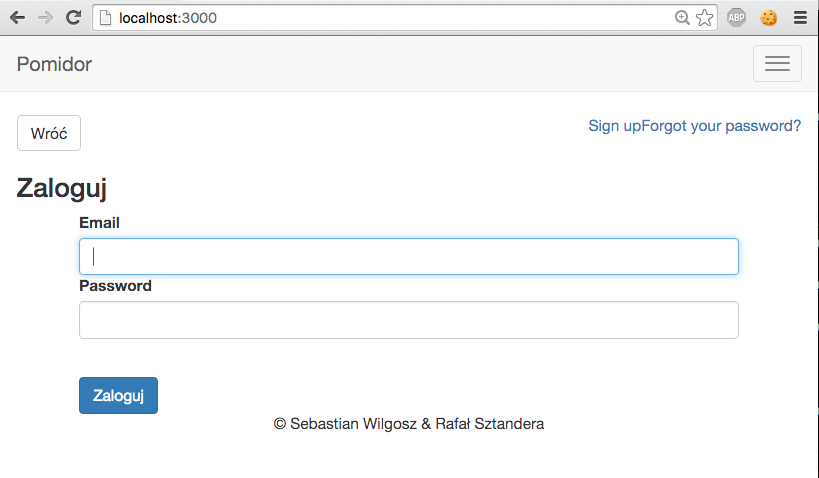
\includegraphics[scale=0.35]{images/root-page-server.png}
  \caption{Widok strony głównej aplikacji}
  \label{figure:root-page-server}
\end{figure}
\FloatBarrier



  \chapter{Implementacja}
  \label{chapter:implementation}
  Kompletne repozytorium aplikacji jest dostępne pod adresem: \url{https://github.com/pwr-wilgosz/pomidor}, poniżej przedstawiliśmy najważniejsze założenia i sposoby implementacji konkretnych rozwiązań.


    \section{Implementacja aplikacji serwerowej}
    \label{section:server}
    \input{server}

    \section{Implementacja aplikacji rpi}
    \label{section:rpi}
    

Stworzenie aplikacji zarządzającej zadaniami
Stworzenie mechanizmu synchronizacji: serwer - aplikacja.
Stworzenie części serwerowej: obsługa komunikacji i odwzorowanie funkcji aplikacji w środowisku webowym



  \chapter{Dostarczone API}
  \label{chapter:api}
  Poniżej zamieszczona została szczegółowa dokumentacja zaimplementowanego API. Każda sekcja składa się z przykładowego zapytania do serwera, listy wymaganych argumentów, które należy przekazać przez URL, możliwe statusy odpowiedzi, które może wysłać serwer, oraz szczegółową odpowiedzią przykładową serwera.

Każdy obiekt JSON zawiera klucz główny, definiujący typ zwracanego modelu, wewnątrz którego zdefiniowane są jego atrybuty.

    \section{Obsługa błędów}
    \label{section:api-errors}
    Poniżej znajduje się lista akceptowanych przez serwer zapytań od aplikacji, oraz lista zwracanych obiektów w formacie JSON.

Serwer nie powinien zwracać nieprzechwytywanych wyjątków, lecz obiekt JSON z odpowiednim polem statusu oraz odpowiednim opisem błędu:

\subsection{ Forbidden}

Ten błąd zwracany jest w przypadku próby wykonania nieautoryzowanej akcji, np. próby utworzenia listy/zadania bez wcześniejszego zalogowania.

\textbf{Format:}

\begin{lstlisting}
  {
    "message": "You are not authorized to access this resource.",
    "status": 403
  }
\end{lstlisting}

\subsection{ Not found}

Próba odwołania do zasobu nieistniejącego na serwerze.

\textbf{Format:}

\begin{lstlisting}
  {
    "message": "Resource is not found.",
    "status": 404
  }
\end{lstlisting}

\subsection{ Unprocessable entity (422)}

Nieprawidłowy format zapytania, na przykład gdy w parametrach do zadania podamy argumenty bez nazwy obiektu:

\begin{lstlisting}
  {
    "name": "Test 1"
  }
\end{lstlisting}

zamiast:

\begin{lstlisting}
  {
    "task": {
      "name": "Test 1"
    }
  }
\end{lstlisting}

\textbf{Format:}

\begin{lstlisting}
  {
    "message": "Unprocessable entity.",
    "status": 422
  }
\end{lstlisting}

\subsection{ Invalid (unauthorized) (401)}

Autoryzacja jest możliwa, ale się nie udała (przy logowaniu, jeśli podamy nieprawidłowe dane)

\textbf{Format:}

\begin{lstlisting}
  {
    "message": "Incorrect email or password",
    "access_token" : null
    "status": 401
  }
\end{lstlisting}

\subsection{Invalid (406)}

Występuje, gdy nie są spełnione wymogi walidacji, np

\begin{lstlisting}
  {
    "message": "List cannot be saved - please, review the errors below.",
    "list": {
      "errors": {
        "title": [
          "can't be blank",
          "has already been taken, but 'List 2 is available'
        ]
      }
    }
  }
\end{lstlisting}


    \section{Sesje logowania}
    \label{section:sessions}
    \subsection{Logowanie}

Aby zalogować uzytkownika i otrzymać odpowiadający mu klucz dostępu, należy wysłać zapytanie do serwera, przekazując w parametrach email oraz hasło. W przypadku pomyślnego logowania, serwer zwróci kod dostępu, \textit{access\_token}, który od tej pory będzie autoryzował użytkownika.

Każde zapytanie do serwera bez podanego w parametrze klucza dostępu zwróci obiekt JSON odpowiadający błędowi (403) \ref{section:api-errors}


\begin{lstlisting}
  POST http://tomato-cal.herokuapp.com/login.json
\end{lstlisting}

Wymagane parametry:
\begin{itemize}
  \item email
  \item password
\end{itemize}

Statusy odpowiedzi:
\begin{itemize}
  \item 200 - ok
  \item 403 - unauthorised
\end{itemize}

\subsubsection{Odpowiedzi:}

Poprawna (200)
\begin{lstlisting}
  {
      "status": 200,
      "access_token" : "abcdefgh"
  }
\end{lstlisting}

Nieprawidłowe dane logowania (403)
\begin{lstlisting}
  {
    "message" : "Invalid email or password",
    "status": 403
  }
\end{lstlisting}


    \section{Zarządzanie listami}
    \label{section:lists}
    \subsection{Pobranie list zadań:}

Założenie jest takie, że każdy użytkownik ma dostęp wyłącznie do swoich list.

\begin{lstlisting}
  GET http://tomato-cal.herokuapp.com/lists?access_token="abc23@klj1309"
\end{lstlisting}

Wymagane argumenty:

\begin{itemize}
  \item access\_token - token identyfikujący użytkownika
\end{itemize}

Statusy:
\begin{itemize}
  \item 200 - ok
  \item 403 - not authorized
\end{itemize}


\subsubsection{Odpowiedzi:}


Poprawna (200) - zwracana jest tablica list wraz z tablicami zadań danej listy
\begin{lstlisting}
  {
    "lists_count": 9,
    "lists": [
      {
        "id": 1,
        "user_id": 1,
        "name": "This is sample list",
        "identifier": "serv_cklsjef323sd3"
        "created_at": "2013-05-30T13:47:41Z",
        "updated_at": "2013-05-30T13:47:41Z"
      }
    ]
  }
\end{lstlisting}

\subsection{Pobranie pojedynczej listy zadań:}

\begin{lstlisting}
  GET http://tomato-cal.herokuapp.com/lists/1?access_token="abc23@klj1309"
\end{lstlisting}

Wymagane argumenty:
\begin{itemize}
  \item access\_token - token identyfikujący użytkownika
  \item id - id identyfikujące daną listę
\end{itemize}

Statusy:
\begin{itemize}
  \item itemize 200 - ok
  \item itemize 403 - not authorized
\end{itemize}

\subsubsection{Odpowiedzi:}
Poprawna (200) - zwracana jest pojedyncza lista wraz z tablicą zadań.
\begin{lstlisting}

  {
    "list":
      {
        "id": 1,
        "user_id": 1,
        "user": {
          "id"=>1,
          "created_at"=>"2015-11-22T15:47:22.701Z",
          "updated_at"=>"2015-11-22T15:47:22.768Z",
          "email"=>"email1@example.com"
        }
        "name": "This is sample list",
        "identifier": "serv_cklsjef323sd3"
        "created_at": "2013-05-30T13:47:41Z",
        "updated_at": "2013-05-30T13:47:41Z"
        "tasks": [
          {
            "id: 1,
            "name: "Task 1",
            "identifier": "serv_cklsjef323sd3",
            "description": "Sample Text",
            "priority": 3,
            "duration": 2,
            "position_x": 12,
            "position_y": 84
          }
        ]
      }
  }
\end{lstlisting}


\subsection{Tworzenie listy}

\begin{lstlisting}
  POST http://tomato-cal.herokuapp.com/lists.json
\end{lstlisting}

Wymagane argumenty
\begin{itemize}
  \item access\_token - token identyfikujący użytkownika§
  \item name - unikalny tytuł
\end{itemize}

Statusy:

\begin{itemize}
  \item 200 - ok
  \item 403 - forbidden
  \item 406 - not acceptable - validation error
\end{itemize}

\subsubsection{Odpowiedzi:}

Correct (201)
\begin{lstlisting}

  {
    "list":
      {
        "id": 1,
        "user_id": 1,
        "user": {
          "id"=>1,
          "created_at"=>"2015-11-22T15:47:22.701Z",
          "updated_at"=>"2015-11-22T15:47:22.768Z",
          "email"=>"email1@example.com"
        }
        "name": "This is sample list",
        "identifier": "serv_cklsjef323sd3"
        "created_at": "2013-05-30T13:47:41Z",
        "updated_at": "2013-05-30T13:47:41Z"
        "tasks": []
      }
  }
\end{lstlisting}


    \section{Zarządzanie zadaniami}
    \label{section:tasks}
    \subsection{Pobranie zadań danej listy:}

Założenie jest takie, że każdy użytkownik ma dostęp wyłącznie do swoich zadań.


\begin{lstlisting}
  GET http://tomato-cal.herokuapp.com/lists/1/tasks?access_token="abc23@klj1309"
\end{lstlisting}


Wymagane argumenty
\begin{itemize}
  \item access\_token - token identyfikujący użytkownika
  \item list\_id - identyfikacja listy
\end{itemize}

Statusy:
\begin{itemize}
  \item 200 - ok
  \item 403 - not authorized
\end{itemize}

\subsubsection{Odpowiedzi:}

Poprawna (200) - zwracana jest tablica zadań

\begin{lstlisting}
  {
   "tasks_count": 9,
    "tasks": [
      {
        "id" => 1,
        "name" => "Test task",
        "priority"=> 1,
        "created_at"=>"2015-11-22T15:47:22.701Z",
        "updated_at"=>"2015-11-22T15:47:22.768Z",
        "identifier" => "serv_llopY8Kz",
        "x"=> 104,
        "y"=> 45,
        "duration" => 3,
        "list_id" => 1
      }
    ]
  }
\end{lstlisting}

\subsection{Pobranie pojedynczego zadania:}

\begin{lstlisting}
    GET http://tomato-cal.herokuapp.com/lists/1/tasks/1?access_token="abc23@klj1309"
\end{lstlisting}

Wymagane argumenty
\begin{itemize}
  \item access\_token - token identyfikujący użytkownika
  \item list\_id - id identyfikujące daną listę
  \item id - id identyfikujące dane zadanie
\end{itemize}

Statusy:
\begin{itemize}
  \item 200 - ok
  \item 403 - not authorized
\end{itemize}

\subsubsection{Odpowiedzi:}

Poprawna (200) - zwracane jest pojedyncze zadanie.

\begin{lstlisting}
  {
    "task" => {
      "id" => 1,
      "name" => "Test task",
      "priority"=> 1,
      "created_at"=>"2015-11-22T15:47:22.701Z",
      "updated_at"=>"2015-11-22T15:47:22.768Z",
      "identifier" => "serv_13llzyI2k",
      "x"=> 104,
      "y"=> 45,
      "duration" => 3,
      "list_id" => 1,
      "list" => {
        "id"=>1,
        "name"=>"Test list",
        "identifier"=>"serv_13llzyI2k",
        "created_at"=>"2015-11-22T15:47:22.701Z",
        "updated_at"=>"2015-11-22T15:47:22.768Z",
        "user_id"=>1
      }
    }
  }
\end{lstlisting}


\subsection{Tworzenie zadania}

\begin{lstlisting}
    POST http://tomato-cal.herokuapp.com/lists/1/tasks.json
\end{lstlisting}

Wymagane argumenty
\begin{itemize}
  \item access\_token - token identyfikujący użytkownika
  \item title - unikalny tytuł
  \item list\_id - identifikator listy
\end{itemize}

Statusy:
\begin{itemize}
  \item 201 - created
  \item 403 - forbidden
  \item 406 - not acceptable - validation error
\end{itemize}

\subsubsection{Odpowiedzi:}

Poprawna (201)
\begin{lstlisting}
  {
    "task" => {
      "id" => 1,
      "name" => "Test task",
      "priority"=> 1,
      "created_at"=>"2015-11-22T15:47:22.701Z",
      "updated_at"=>"2015-11-22T15:47:22.768Z",
      "identifier" => "serv_13llzyI2k",
      "x"=> 104,
      "y"=> 45,
      "duration" => 3,
      "list_id" => 1,
      "list" => {
        "id"=>1,
        "name"=>"Test list",
        "identifier"=>"serv_13llzyI2k",
        "created_at"=>"2015-11-22T15:47:22.701Z",
        "updated_at"=>"2015-11-22T15:47:22.768Z",
        "user_id"=>1
      }
    }
  }
\end{lstlisting}


    \section{Synchronizacja}
    \label{section:sync}
    Aby zsynchronizować bazy, należy wykonać zapytanie:

\begin{lstlisting}

    GET http://tomato-cal.herokuapp.com/sync
\end{lstlisting}

Wymagane argumenty:

\begin{itemize}
  \item access\_token - token identyfikujący użytkownika
  \item snapshot - obraz bazy danych na urządzeniu: kolekcja wszystkich list i zadań.
\end{itemize}

Przykład:

\begin{lstlisting}
curl -H 'Content-Type: application/json' -H 'Accept: application/json' -X POST http://tomato-cal.herokuapp.com/sync?access_token=42fF2zhLai3 -d '
  {
    lists: [
      {
        identifier: "rpi_4LK3kll2nza",
        name: "Test list",
        updated_at: "2013-05-30T13:47:41Z",
        tasks: [
          {
            "name" => "Test task",
            "priority"=> 1,
            "updated_at"=>"2015-11-22T15:47:22.768Z",
            "identifier" => 'rpi_0v9Kds2ngi',
            "x"=> 104,
            "y"=> 45,
            "duration" => 3
          }
        ]
      }
    ]
  }'

\end{lstlisting}

Statusy:

\begin{itemize}
  \item 200 - ok
  \item 403 - not authorized
\end{itemize}

Odpowiedzi:

Poprawna (200) - zwracana jest zsynchronizowana tablica list wraz z tablicami zadań danej listy

\begin{lstlisting}
  {
    lists: [
      {
        id: 1,
        identifier: "rpi_4LK3kll2nza",
        name: "Test list",
        created_at: "2013-05-30T13:47:41Z",
        updated_at: "2013-05-30T13:47:41Z",
        tasks: [
          {
            "id" => 1,
            "name" => "Test task",
            "priority"=> 1,
            "created_at"=>"2015-11-22T15:47:22.701Z",
            "updated_at"=>"2015-11-22T15:47:22.768Z",
            "identifier" => task.identifier,
            "x"=> 104,
            "y"=> 45,
            "duration" => 3,
            "list_id" => 1
          }
        ]
      }
    ]
  }
\end{lstlisting}


  \chapter{Wnioski}
  \label{chapter:conclusions}
  W niniejszej pracy został opisany proces przygotowania systemu wybudowanego opartego na koncepcji Internet of Things.
Przedstawiono narzędzia umożliwiające zaprojektowanie, i wytworzenie takiego systemu, wraz z wyjaśnieniem decyzji podejmowanych przy wyborze poszczególnych. Opisane zostały również wybrane koncepcje wytwarzania oprogramowania i oraz autorska metoda synchronizacji danych przy użyciu asynchronicznych zapytań RESTowych oraz obiektów JSON.

Część praktyczna pracy składa się z urządzenia odpowiednio skonfigurowanego do pracy z wyświetlaczem dotykowym, aplikacji mobilnej, która  łączy w sobie wszystkie założone funkcjonalności takie jak możliwość dodawania i zarządzania listami zadań, możliwością porządkowania zadań według priorytetów oraz sterowanie wykonywaniem zadań (czasomierz). Zaimplementowany został mechanizm synchronizacji oraz aplikacja webowa. Całość tworzy system, który dowodzi spełnienia postawionych założeń oraz prezentuje przykładowe zastosowanie systemu z użyciem platformy mikroprocesorowej - w tym przypadku - systemu wspomagającego zarządzaniem czasem i zadaniami.

Podczas projektowania systemu autorzy nie przewidzieli, że zastosowane rozwiązanie - zestaw bibliotek Kivy obsługujące część graficzną aplikacji - nie będzie odbsługiwane przez wbudowaną w urządzenie (Raspberry Pi) kartę graficzną. Bez wspomagania sprzętowego aplikacja działa bardzo wolno. W najnowszym wydaniu, producent Kivy zapowiedział wsparcie dla tego urządzenia.

Podsumowując, współczesna technologia umożliwia tworzenie oprogramowania użytkowego, które może w pełni integrować się z istniejącymi systemami wbudowanymi takimi jak składowe iteligentnego domu, czy urządzeń zaprojektowanych według koncepcji Internet of Things. Stworzenie systemu rozproszonego według opisanego w pracy rozwiązania wymaga niewielkiego nakładu finansowego i czasowego. Spektrum rozwiązań jakie podobne systemy mogą oferować, jest bardzo duże i zróżnicowane, podobnie jak to ma miejsce w przypadku aplikacji mobilnych dedykowanych dla wybranych producentów systemów operacyjnych.

\begin{figure}[ht]
  \centering
  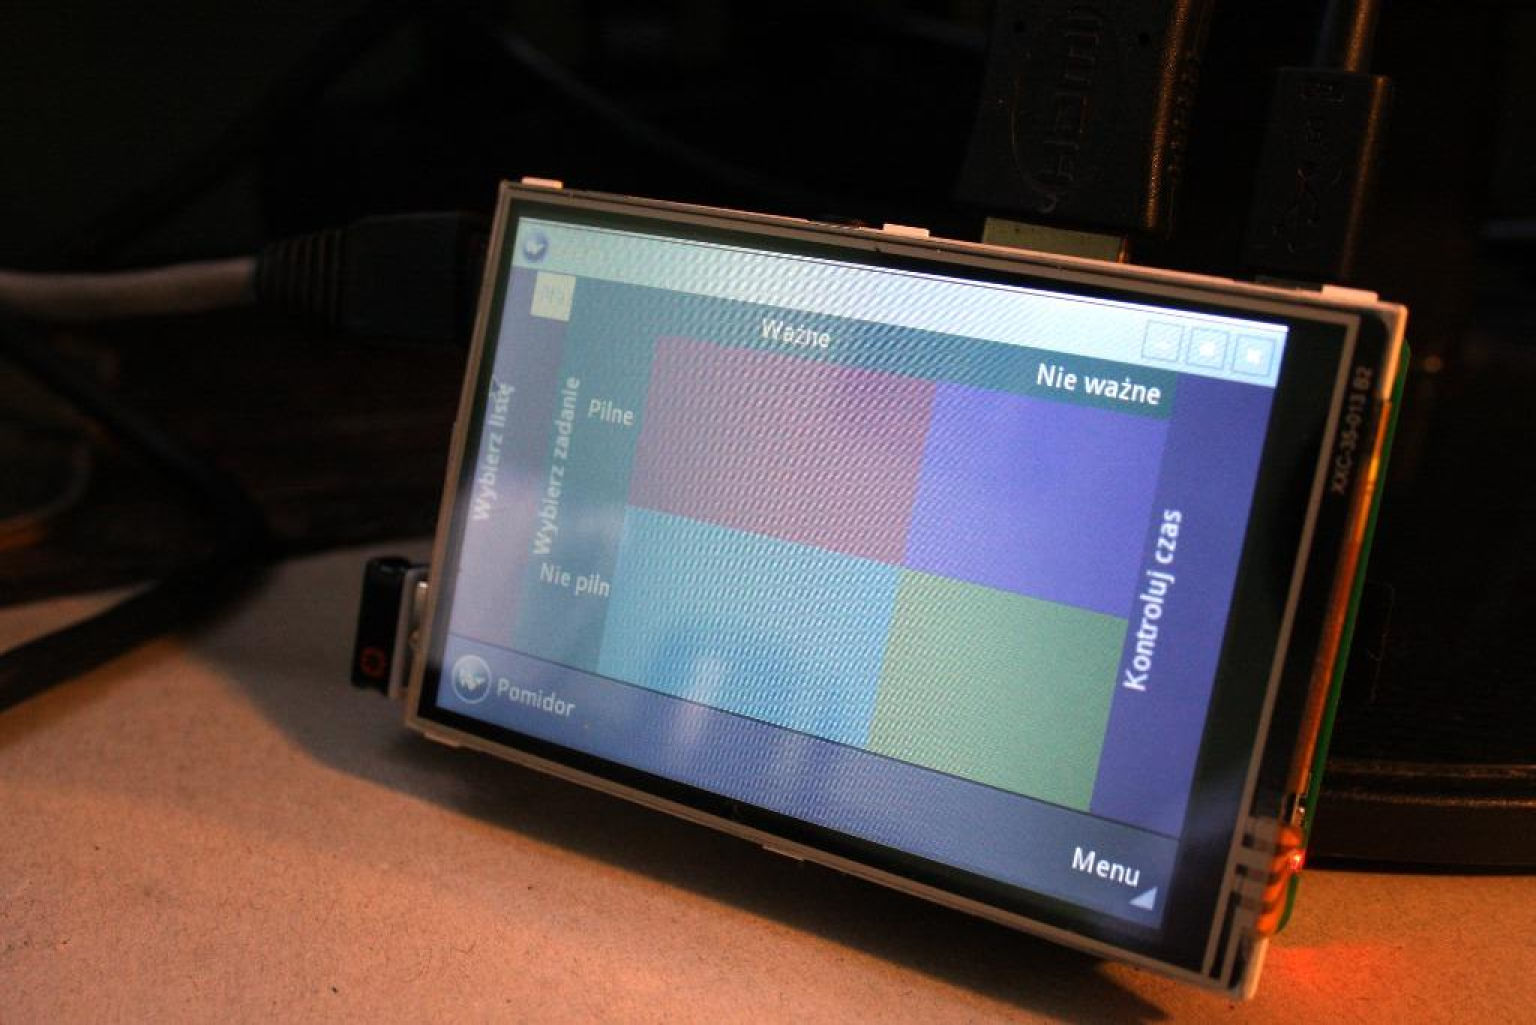
\includegraphics[width=\textwidth]{images/przyklad.png}
  \caption{Aplikacja zainstalowana na urządzeniu}
  \label{figure:przykladowa_app}
\end{figure}


  \begin{thebibliography}{plain}
    \label{bibliography}
    \bibitem{bib:mobile-challenge} Mizouni, R.; Serhani, A. ; Dssouli, R. ; Benharref, A.: Back to Results Challenges in “mobilizing” desktop applications: a new methodology for requirements engineering,  Coll. of Inf. Technol., UAE Univ., Al-Ain, United Arab Emirates, 2009

\bibitem{bib:mobile-paradigm} Ngu Phuc Huy; Do Van Thanh: Selecting the right mobile app paradigms Dept. of Telematics, Norwegian Univ. of Sci. \& Technol., Trondheim, Norway, 2012

\bibitem{bib:iot-middleware}Razzaque, M.A.; Milojevic-Jevric, M. ; Palade, A. ; Clarke, S.: Middleware for Internet of Things: a Survey,  Trinity College Dublin, Dublin, Ireland.

\bibitem{bib:mgr-rpi} Chi Winth Ea; Morten Sørbø: Multi-purpose Embedded Communication Gateway: System Design and Testbed Implementation, University of Agder, 2014

\bibitem{bib:xhr} Adeyeye, M.; Makitla, I. ; Fogwill, T.: Determining the signalling overhead of two common WebRTC methods: JSON via XMLHttpRequest and SIP over WebSocket, Dept. of Inf. Technol., Cape Peninsula Univ. of Technol., Cape Town, South Africa, 2013

\bibitem{bib:ruby-doc} Dokumentacja języka Ruby, \url{https://www.ruby-lang.org/en/}

\bibitem{bib:rails-doc} Dokumentacja Ruby on rails, \url{http://guides.rubyonrails.org/}

\bibitem{bib:coffeescript-doc} Dokumentacja CoffeeScript, \url{http://coffeescript.org/}

\bibitem{bib:sass-doc} Dokumentacja Sass, \url{http://sass-lang.com/}

\bibitem{bib:jquery-doc} Dokumentacja biblioteki jQuery, \url{https://jquery.com/}

\bibitem{bib:rvm-install} Opis instalacji RVM (Ruby Version Manager), \url{https://rvm.io/rvm/install }

  \end{thebibliography}

\end{document}
